% Gemini theme
% https://github.com/anishathalye/gemini

\documentclass[final,notheorems]{beamer}

% ====================
% Packages
% ====================

\usepackage[T1]{fontenc}
\usepackage{lmodern}
\usepackage[size=a0,scale=1.0]{beamerposter}
% \usepackage[size=custom,width=120,height=72,scale=1.0]{beamerposter}
\usetheme{gemini}
\usecolortheme{ppposter}
\usepackage{graphicx}
\usepackage{booktabs}
\usepackage{tikz}
\usepackage{pgfplots}
\usepackage{amsmath}
\usepackage[backend=biber,maxcitenames=4,maxbibnames=99,giveninits=false]{biblatex}
\usepackage{xcolor}
\usepackage{siunitx}
\usepackage{wrapfig}
\usepackage{bm}
\setbeamertemplate{theorems}[numbered] % to number

\addbibresource{poster.bib}

% ====================
% Lengths
% ====================

% If you have N columns, choose \sepwidth and \colwidth such that
% (N+1)*\sepwidth + N*\colwidth = \paperwidth
\newlength{\sepwidth}
\newlength{\colwidth}
\setlength{\sepwidth}{0.025\paperwidth}
\setlength{\colwidth}{0.3\paperwidth}

\newcommand{\separatorcolumn}{\begin{column}{\sepwidth}\end{column}}

% ====================
% Commands
% ====================
\providecommand{\abs}[1]{\lvert#1\rvert}
\providecommand{\norm}[1]{\lVert#1\rVert}
\DeclareBoldMathCommand\bfx{x}
\DeclareBoldMathCommand\bfv{v}
\def\X{\mathcal X}
\def\R{\mathbb R}
\def\deq{\stackrel{{\mathrm d}}{=}}

\newtheorem{imp}{Implication}

\definecolor{highlightbg}{HTML}{fcd588}


% ====================
% Title
% ====================

\title{Human Perception of Adversarial Images}

\author{Ayon Sen \inst{1} \and Xiaojin Zhu \inst{1} \and Liam Marshall \inst{1} \and Robert Nowak \inst{1}}

\institute[shortinst]{\inst{1} University of Wisconsin-Madison}

\addtobeamertemplate{headline}{}
{
    \begin{tikzpicture}[remember picture,overlay]
    \node [anchor=north east, inner sep=2cm] at ([xshift=1.4cm,yshift=1.2cm]current page.north east)     {
\includegraphics[height=6.5cm]{fig/black-flush-UWlogo-print.eps}};
    \end{tikzpicture}
}
% ====================
% Body
% ====================

\begin{document}

\begin{frame}[t]
\begin{columns}[t]
\separatorcolumn

\begin{column}{\colwidth}
  \begin{block}{Overview}
    \begin{wrapfigure}{R}{.40\textwidth}
      \centering
      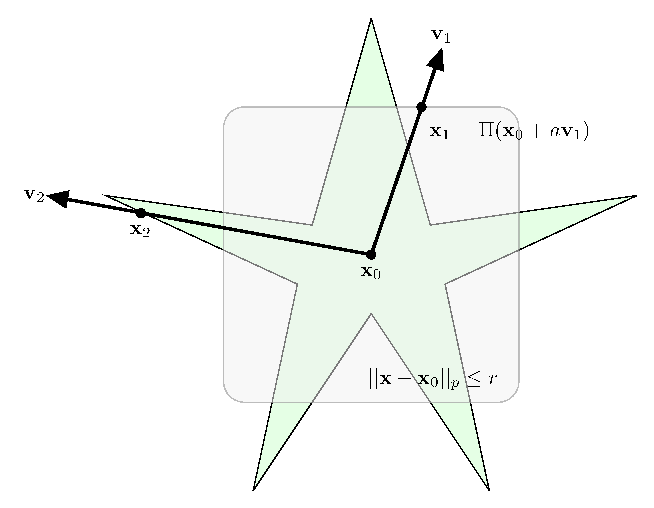
\includegraphics[width=0.38\textwidth]{fig/intro_image-figure0.eps}
      \caption{Current research assumes a $p$-norm decision boundary (grey) on whether an image has been tampered with. The true human decision boundary (green) may be very different.}
      \label{fig:decision_boundary}
    \end{wrapfigure}
    Adversarial attacks attempt to confound machine learning systems. By changing the input to a classifier slightly -- for instance, tweaking image pixels -- the output classification can be manipulated.

    Throughout the literature on attacking image classifiers, the \emph{visibility} of attacks to a human observer (who might become \emph{suspicious}, which we wish to avoid) is typically gauged (without adequate justification) by a $p$-norm of the difference between the original and modified image.

    Via behavioral experiments, we show~\cite{sen2019perception} that \textbf{human perception of image modifications is not well-described by \emph{any} $p$-norm, nor several alternative measures}.
    This has significant impact on adversarial ML research; the robustness of attacks to human inspection relies on an accurate understanding of \emph{what humans will and will not see as "tampering"}.

  \end{block}

  \begin{alertblock}{The current assumption}
    An image $\bfx_0$ sits in a pixel feature space $\X = \{0,\ldots,255\}^d$, where $d$ = $\text{\# pixels} \times \text{\# color channels}$ (assuming a color depth of 255).

    An adversarial attack perturbs this $\bfx_0$ into $\bfx$. Currently, the \textbf{general assumption} in adversarial image attacks is that:

    \hspace*{.1\linewidth}\colorbox{highlightbg}{\begin{minipage}{.8\linewidth}
      There exists some global $p>0$ and some $r$ (dependent on $\bfx_0$) where the observer perceives all $\bfx$ as visually identical to $\bfx_0$ as long as $\norm{\bfx_0-\bfx}_p < r(x_0)$ is satisfied.
    \end{minipage}}

    We refute this assumption via \emph{testable implications}.
  \end{alertblock}

  \begin{block}{A weak implication}
    We define $J(\bfx_0) = \{\bfx \subset \X : \norm{\bfx_0-\bfx}_p = r(\bfx_0)\}$ as the set of all images just-noticeably-different from the base image $\bfx_0$.

    \hspace*{.1\linewidth}\colorbox{highlightbg}{\begin{minipage}{.8\linewidth}
      Supposing $p^*$ is the true value of $p$, for any pair of $\bfx_1$, $\bfx_2$ $\in J(\bfx_0)$, $\norm{\bfx_1-\bfx_0}_{p^*} = \norm{\bfx_2-\bfx_0}_{p^*}$.
    \end{minipage}}

    We can ask humans when they 'just notice' changes to an image and compare these judgments across $\bfx_1$, $\bfx_2$ pairs, but this implication is still \emph{weak} as a statistical test; it \emph{requires knowledge of the true $p^*$}.
  \end{block}

  \begin{block}{A stronger implication}
    Throughout our experiments, we generate images as in Figure~\ref{fig:decision_boundary};
    each image $\bfx = \Pi(\bfx_0+a\bfv)$ is defined by a ray or \textbf{perturbation direction} $\bfv \in \R^d$ and a \textbf{perturbation scale} $a>0$.
    $\Pi$ is the projection onto $\X$ (clipping and rounding).

    We construct \textbf{$\pm 1$-perturbation directions} as $\bfv\in\R^d$ where
    (i) $\bfv$ has $s>0$ nonzero elements, and
    (ii) $v_i = 1$ if $v_0,i < 128$ and $=-1$ otherwise.

    It is then possible to extract a new implication, testable without knowledge of $p^*$:

    \hspace*{.1\linewidth}\colorbox{highlightbg}{\begin{minipage}{.8\linewidth}
      If two perturbation directions $\bfv_1$, $\bfv_2$ have the same sparsity $s$, the perturbation scales $a_1$, $a_2$ at which humans notice changes must be equal.
    \end{minipage}}
  \end{block}

    \begin{block}{Designing Perturbations}
    Our three $\bfx_0$s were (cat, panda, macaw) from Imagenet. We empirically defined a set of designed perturbations that would showcase inconsistencies in norms, and generated eight of those per $\bfx_0$ (see Table~\ref{tab:rays}), plus two FGSM and PGD adversarial attack rays for each image (with arbitrary target labels).
    \begin{table}
        \centering
          \begin{small}
            \begin{tabular}{l|l|l}
              \multicolumn{1}{c|}{\textbf{\# Dimensions Changed (s)}} & \multicolumn{1}{c|}{\textbf{Color Channels Affected}} & \multicolumn{1}{c}{\textbf{Shape of Perturbed Pixels}} \\\hline
              S = 1, M = 288 & Red = only the red channel of a pixel & Box = a centered rectangle \\
              L = 30603, X = 268203 & RGB = all three channels of a pixel & Dot = scattered random dots \\
              (mnemonic: garment size) & & Eye = on the eye of the animal \\
            \end{tabular}
          \end{small}
        \caption{$\pm1$-perturbation directions varying in size, number of color channels affected, and shape of perturbed pixels}
        \label{tab:rays}
    \end{table}

  \end{block}
\end{column}

\separatorcolumn

\begin{column}{\colwidth}

  \begin{block}{Experimental design}
    68 Amazon Mechanical Turk workers were presented with instructions and then completed a sequence of 34 trials, 30 of which were $\pm1$-perturbation or adversarial trials,
    and 4 of which were "guard trials", with an abrupt change to filter out participants clicking through without performing the task.

    \begin{figure}
      \centering
      \includegraphics[width=\linewidth]{fig/temporal_diagram-figure0.eps}
      \caption{Experiment procedure.
      The green, red and blue cells denote $\pm 1$-perturbation, adversarial, and guard trials, respectively.
      The letters P, M and C denote the panda, macaw and cat $\bfx_0$, respectively.
      }
      \label{fig:temporal}
    \end{figure}

    Each trial consisted of stepping along a perturbation ray $\bfv$, using arrow keys or buttons to increment/decrement $a$ by 1.
    The user was instructed to submit immediately when they noticed a difference in the image.
    We saved the final $a$ submitted by the user for each $(\bfx_0, \bfv)$ pair, as well as their path over time to reach that $a$.
    For $\pm1$-perturbation trials, $a$ was constrained $\in\{0,1,\ldots,128\}$ to avoid value clipping. Users were encouraged to "give up" at $a=128$ (producing right-censored data).

  \end{block}

  \begin{block}{Analysis}
    Since our participants were not ideal observers, we treat the pool of all returned responses for some $(\bfx_0, \bfv)$ pair as a sample.
\begin{figure}[h]
  \begin{center}
    \begin{tabular}{ccc}
      $p=1,\ \bfx_0=\text{panda}$ & $p=2,\ \bfx_0=\text{macaw}$ & $p=\infty,\ \bfx_0=\text{cat}$ \\
      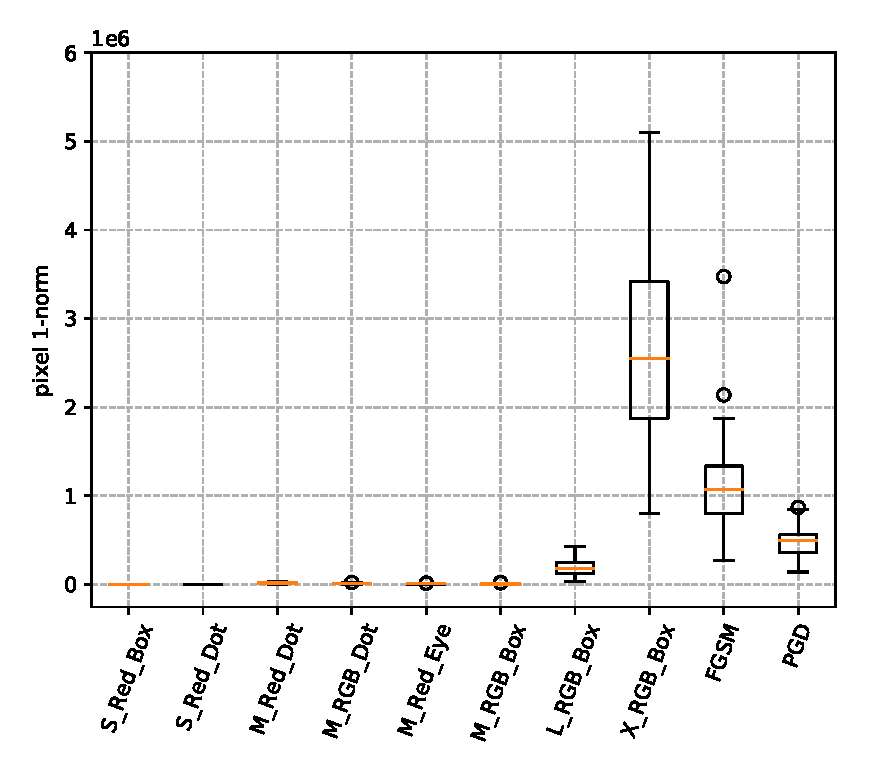
\includegraphics[width=0.3\textwidth]{fig/pixel_1_norm_boxplot_panda.eps} &
      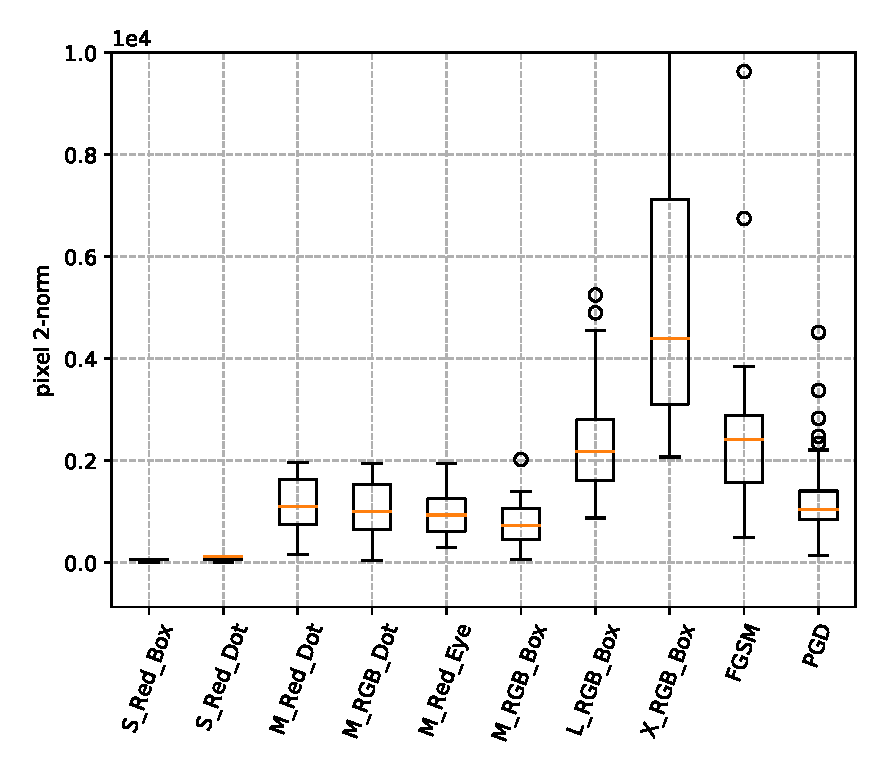
\includegraphics[width=0.3\textwidth]{fig/pixel_2_norm_boxplot_macaw.eps} &
      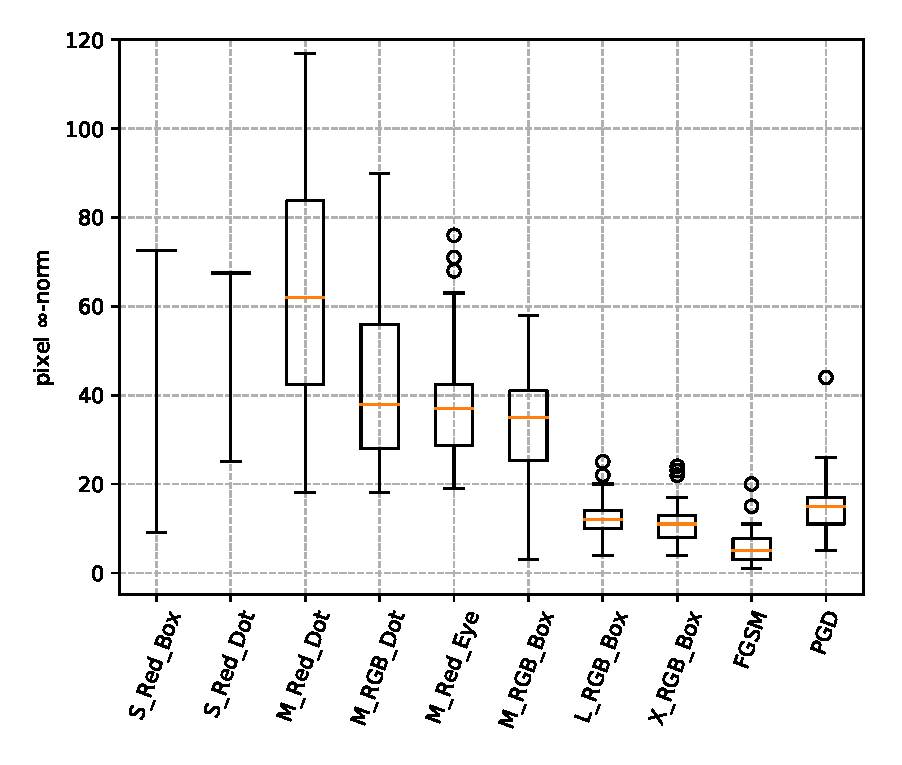
\includegraphics[width=0.3\textwidth]{fig/pixel_inf_norm_boxplot_cat.eps} 
    \end{tabular}
  \end{center}
  \caption{Distribution of norms ($p$ varies) over all responses of image changes at the just-noticable point. If the central hypothesis were true, each plot should locally have similar medians (orange lines).}
  \label{fig:Lp_excerpt}
\end{figure}


    We perform Kolmogorov-Smirnov non-parametric distribution equality tests over these samples to check implications. Let $x_1^{(j)}$ be user $j$'s just-noticeable image along ray $\bfv_1$. Note that $a_1^{(j)} \deq a_2^{(j)}$ corresponds to the strong implication $s_1=s_2\Rightarrow a_1=a_2$.
  \end{block}
\end{column}

\separatorcolumn

\begin{column}{\colwidth}
  \begin{block}{Statistical Tests}
    Testing the weaker implication: \textbf{1, 2, $\infty$-norms do not accurately describe our data.} \\
    
    \[H_0 : \norm{\bfx_1^{(j)} - \bfx_0}_p \deq  \norm{\bfx_2^{(j)}}_p\]
    \begin{table}
      \centering
      \begin{tabular}{c | l l l | c}
        $p$-norm & $\bfx_0$ & $\bfv_1$ & $\bfv_2$ & \textbf{\textit{p}} \\
        \midrule
        1 & \texttt{panda} & \texttt{FGSM} & \texttt{M-RGB-Dot} & \num{6.4e-19} \\
        2 & \texttt{macaw} & \texttt{PGD} & \texttt{X-RGB-Box} & \num{2.6e-16} \\
        $\infty$ & \texttt{cat} & \texttt{M-RGB-Box} & \texttt{L-RGB-Box} & \num{1.1e-14} \\
      \end{tabular}
      \caption{Hypothesis instances and \emph{statistical} $p$-values (2-sample KS test). Note each test uses different $\bfx_0$, $\bfv_1$, $\bfv_2$.}
    \end{table}

    Testing the stronger implication: \textbf{no $p$-norm accurately fits the human responses.}

    \[H_0 : a_1^{(j)} \deq a_2^{(j)}\]
    \begin{table}
      \centering
      \begin{tabular}{l l l | c}
        $\bfx_0$ & $\bfv_1$ & $\bfv_2$ & \textbf{\textit{p}} \\
        \midrule
        \texttt{cat} & \texttt{M-Red-Dot} & \texttt{M-Red-Eye} & \num{9.5e-6} \\
        \texttt{panda} & \texttt{M-Red-Dot} & \texttt{M-RGB-Dot} & \num{2.1e-4} \\
      \end{tabular}
      \caption{Hypothesis instances and \emph{statistical} $p$-values (2-sample KS test).}
    \end{table}

    \begin{figure}
      \centering
      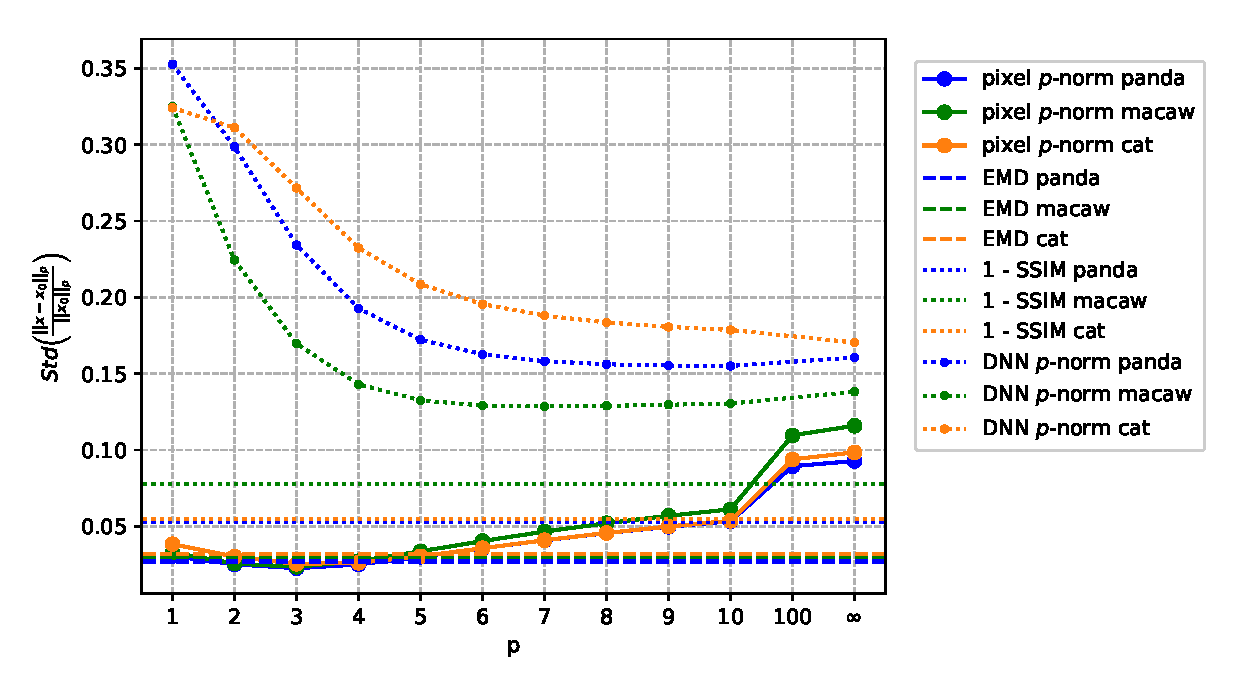
\includegraphics{fig/best_p_approx2.eps}
      \caption{Variability of fit to human data for various measures (lower is better).}
      \label{fig:fit}
    \end{figure}


    In Fig~\ref{fig:fit}, results from several other distance measures ($p$-norm on a neural-network derived representation of the image, SSIM structural similarity, and earthmover's distance) are shown against pixel $p$-norms for various values of $p$.

  \end{block}

  \begin{alertblock}{Conclusion}

  \end{alertblock}

  \begin{block}{References}
    \footnotesize{\printbibliography}
  \end{block}

\end{column}

\separatorcolumn
\end{columns}
\end{frame}

\end{document}
